% Created by tikzDevice version 0.10.1 on 2018-02-17 17:13:00
% !TEX encoding = UTF-8 Unicode
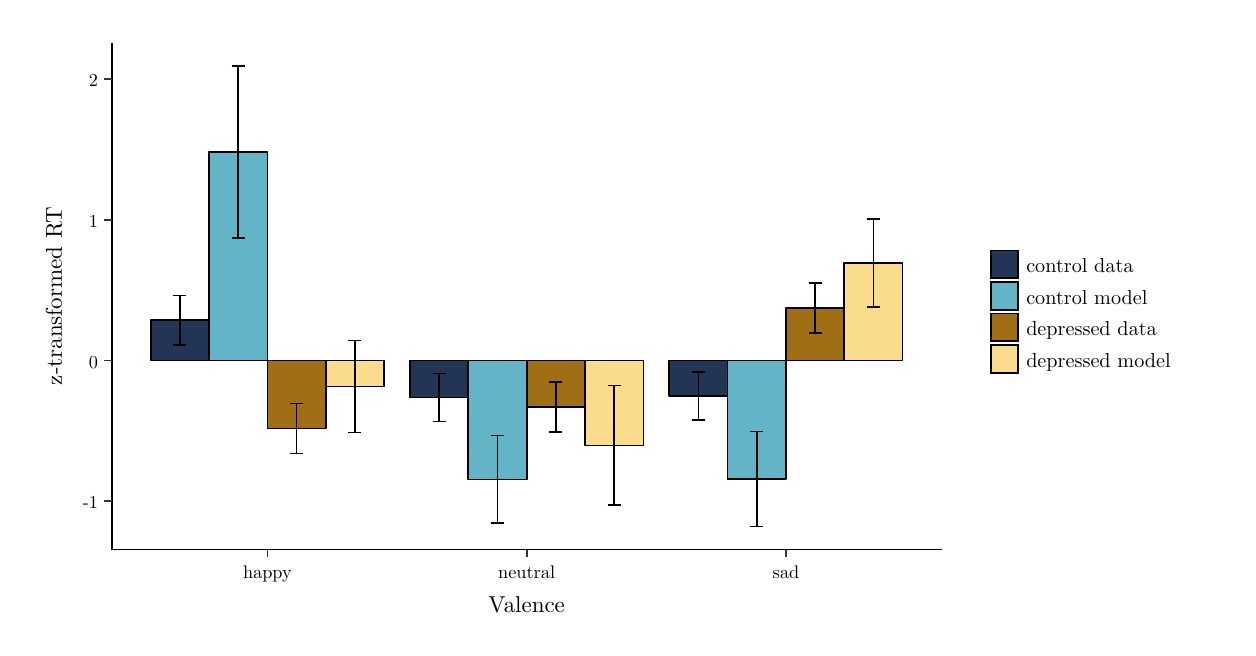
\begin{tikzpicture}[x=1pt,y=1pt]
\definecolor{fillColor}{RGB}{255,255,255}
\path[use as bounding box,fill=fillColor,fill opacity=0.00] (0,0) rectangle (433.62,216.81);
\begin{scope}
\path[clip] (  0.00,  0.00) rectangle (433.62,216.81);
\definecolor{drawColor}{RGB}{255,255,255}
\definecolor{fillColor}{RGB}{255,255,255}

\path[draw=drawColor,line width= 0.6pt,line join=round,line cap=round,fill=fillColor] (  0.00,  0.00) rectangle (433.62,216.81);
\end{scope}
\begin{scope}
\path[clip] ( 30.40, 28.22) rectangle (330.22,211.31);
\definecolor{fillColor}{RGB}{255,255,255}

\path[fill=fillColor] ( 30.40, 28.22) rectangle (330.22,211.31);
\definecolor{drawColor}{RGB}{0,0,0}
\definecolor{fillColor}{RGB}{250,220,140}

\path[draw=drawColor,line width= 0.6pt,line join=round,fill=fillColor] (107.69, 87.12) rectangle (128.77, 96.53);
\definecolor{fillColor}{RGB}{160,110,20}

\path[draw=drawColor,line width= 0.6pt,line join=round,fill=fillColor] ( 86.61, 72.01) rectangle (107.69, 96.53);
\definecolor{fillColor}{RGB}{100,180,200}

\path[draw=drawColor,line width= 0.6pt,line join=round,fill=fillColor] ( 65.53, 96.53) rectangle ( 86.61,171.93);
\definecolor{fillColor}{RGB}{35,53,85}

\path[draw=drawColor,line width= 0.6pt,line join=round,fill=fillColor] ( 44.45, 96.53) rectangle ( 65.53,111.13);
\definecolor{fillColor}{RGB}{250,220,140}

\path[draw=drawColor,line width= 0.6pt,line join=round,fill=fillColor] (201.39, 65.87) rectangle (222.47, 96.53);
\definecolor{fillColor}{RGB}{160,110,20}

\path[draw=drawColor,line width= 0.6pt,line join=round,fill=fillColor] (180.31, 79.74) rectangle (201.39, 96.53);
\definecolor{fillColor}{RGB}{100,180,200}

\path[draw=drawColor,line width= 0.6pt,line join=round,fill=fillColor] (159.22, 53.58) rectangle (180.31, 96.53);
\definecolor{fillColor}{RGB}{35,53,85}

\path[draw=drawColor,line width= 0.6pt,line join=round,fill=fillColor] (138.14, 83.14) rectangle (159.22, 96.53);
\definecolor{fillColor}{RGB}{250,220,140}

\path[draw=drawColor,line width= 0.6pt,line join=round,fill=fillColor] (295.08, 96.53) rectangle (316.16,131.73);
\definecolor{fillColor}{RGB}{160,110,20}

\path[draw=drawColor,line width= 0.6pt,line join=round,fill=fillColor] (274.00, 96.53) rectangle (295.08,115.40);
\definecolor{fillColor}{RGB}{100,180,200}

\path[draw=drawColor,line width= 0.6pt,line join=round,fill=fillColor] (252.92, 53.74) rectangle (274.00, 96.53);
\definecolor{fillColor}{RGB}{35,53,85}

\path[draw=drawColor,line width= 0.6pt,line join=round,fill=fillColor] (231.84, 83.72) rectangle (252.92, 96.53);

\path[draw=drawColor,line width= 0.6pt,line join=round] (115.89,103.74) --
	(120.58,103.74);

\path[draw=drawColor,line width= 0.6pt,line join=round] (118.23,103.74) --
	(118.23, 70.50);

\path[draw=drawColor,line width= 0.6pt,line join=round] (115.89, 70.50) --
	(120.58, 70.50);

\path[draw=drawColor,line width= 0.6pt,line join=round] ( 94.81, 81.04) --
	( 99.50, 81.04);

\path[draw=drawColor,line width= 0.6pt,line join=round] ( 97.15, 81.04) --
	( 97.15, 62.98);

\path[draw=drawColor,line width= 0.6pt,line join=round] ( 94.81, 62.98) --
	( 99.50, 62.98);

\path[draw=drawColor,line width= 0.6pt,line join=round] ( 73.73,202.99) --
	( 78.41,202.99);

\path[draw=drawColor,line width= 0.6pt,line join=round] ( 76.07,202.99) --
	( 76.07,140.87);

\path[draw=drawColor,line width= 0.6pt,line join=round] ( 73.73,140.87) --
	( 78.41,140.87);

\path[draw=drawColor,line width= 0.6pt,line join=round] ( 52.65,120.05) --
	( 57.33,120.05);

\path[draw=drawColor,line width= 0.6pt,line join=round] ( 54.99,120.05) --
	( 54.99,102.22);

\path[draw=drawColor,line width= 0.6pt,line join=round] ( 52.65,102.22) --
	( 57.33,102.22);

\path[draw=drawColor,line width= 0.6pt,line join=round] (209.59, 87.48) --
	(214.27, 87.48);

\path[draw=drawColor,line width= 0.6pt,line join=round] (211.93, 87.48) --
	(211.93, 44.26);

\path[draw=drawColor,line width= 0.6pt,line join=round] (209.59, 44.26) --
	(214.27, 44.26);

\path[draw=drawColor,line width= 0.6pt,line join=round] (188.50, 88.74) --
	(193.19, 88.74);

\path[draw=drawColor,line width= 0.6pt,line join=round] (190.85, 88.74) --
	(190.85, 70.74);

\path[draw=drawColor,line width= 0.6pt,line join=round] (188.50, 70.74) --
	(193.19, 70.74);

\path[draw=drawColor,line width= 0.6pt,line join=round] (167.42, 69.46) --
	(172.11, 69.46);

\path[draw=drawColor,line width= 0.6pt,line join=round] (169.77, 69.46) --
	(169.77, 37.71);

\path[draw=drawColor,line width= 0.6pt,line join=round] (167.42, 37.71) --
	(172.11, 37.71);

\path[draw=drawColor,line width= 0.6pt,line join=round] (146.34, 91.83) --
	(151.03, 91.83);

\path[draw=drawColor,line width= 0.6pt,line join=round] (148.68, 91.83) --
	(148.68, 74.46);

\path[draw=drawColor,line width= 0.6pt,line join=round] (146.34, 74.46) --
	(151.03, 74.46);

\path[draw=drawColor,line width= 0.6pt,line join=round] (303.28,147.64) --
	(307.96,147.64);

\path[draw=drawColor,line width= 0.6pt,line join=round] (305.62,147.64) --
	(305.62,115.81);

\path[draw=drawColor,line width= 0.6pt,line join=round] (303.28,115.81) --
	(307.96,115.81);

\path[draw=drawColor,line width= 0.6pt,line join=round] (282.20,124.44) --
	(286.88,124.44);

\path[draw=drawColor,line width= 0.6pt,line join=round] (284.54,124.44) --
	(284.54,106.37);

\path[draw=drawColor,line width= 0.6pt,line join=round] (282.20,106.37) --
	(286.88,106.37);

\path[draw=drawColor,line width= 0.6pt,line join=round] (261.12, 70.93) --
	(265.80, 70.93);

\path[draw=drawColor,line width= 0.6pt,line join=round] (263.46, 70.93) --
	(263.46, 36.55);

\path[draw=drawColor,line width= 0.6pt,line join=round] (261.12, 36.55) --
	(265.80, 36.55);

\path[draw=drawColor,line width= 0.6pt,line join=round] (240.04, 92.41) --
	(244.72, 92.41);

\path[draw=drawColor,line width= 0.6pt,line join=round] (242.38, 92.41) --
	(242.38, 75.04);

\path[draw=drawColor,line width= 0.6pt,line join=round] (240.04, 75.04) --
	(244.72, 75.04);
\end{scope}
\begin{scope}
\path[clip] (  0.00,  0.00) rectangle (433.62,216.81);
\definecolor{drawColor}{RGB}{0,0,0}

\path[draw=drawColor,line width= 0.6pt,line join=round] ( 30.40, 28.22) --
	( 30.40,211.31);
\end{scope}
\begin{scope}
\path[clip] (  0.00,  0.00) rectangle (433.62,216.81);
\definecolor{drawColor}{RGB}{0,0,0}

\node[text=drawColor,anchor=base east,inner sep=0pt, outer sep=0pt, scale=  0.66] at ( 25.45, 42.94) {-1};

\node[text=drawColor,anchor=base east,inner sep=0pt, outer sep=0pt, scale=  0.66] at ( 25.45, 93.81) {0};

\node[text=drawColor,anchor=base east,inner sep=0pt, outer sep=0pt, scale=  0.66] at ( 25.45,144.67) {1};

\node[text=drawColor,anchor=base east,inner sep=0pt, outer sep=0pt, scale=  0.66] at ( 25.45,195.54) {2};
\end{scope}
\begin{scope}
\path[clip] (  0.00,  0.00) rectangle (433.62,216.81);
\definecolor{drawColor}{gray}{0.20}

\path[draw=drawColor,line width= 0.6pt,line join=round] ( 27.65, 45.66) --
	( 30.40, 45.66);

\path[draw=drawColor,line width= 0.6pt,line join=round] ( 27.65, 96.53) --
	( 30.40, 96.53);

\path[draw=drawColor,line width= 0.6pt,line join=round] ( 27.65,147.40) --
	( 30.40,147.40);

\path[draw=drawColor,line width= 0.6pt,line join=round] ( 27.65,198.27) --
	( 30.40,198.27);
\end{scope}
\begin{scope}
\path[clip] (  0.00,  0.00) rectangle (433.62,216.81);
\definecolor{drawColor}{RGB}{0,0,0}

\path[draw=drawColor,line width= 0.6pt,line join=round] ( 30.40, 28.22) --
	(330.22, 28.22);
\end{scope}
\begin{scope}
\path[clip] (  0.00,  0.00) rectangle (433.62,216.81);
\definecolor{drawColor}{gray}{0.20}

\path[draw=drawColor,line width= 0.6pt,line join=round] ( 86.61, 25.47) --
	( 86.61, 28.22);

\path[draw=drawColor,line width= 0.6pt,line join=round] (180.31, 25.47) --
	(180.31, 28.22);

\path[draw=drawColor,line width= 0.6pt,line join=round] (274.00, 25.47) --
	(274.00, 28.22);
\end{scope}
\begin{scope}
\path[clip] (  0.00,  0.00) rectangle (433.62,216.81);
\definecolor{drawColor}{RGB}{0,0,0}

\node[text=drawColor,anchor=base,inner sep=0pt, outer sep=0pt, scale=  0.66] at ( 86.61, 17.82) {happy};

\node[text=drawColor,anchor=base,inner sep=0pt, outer sep=0pt, scale=  0.66] at (180.31, 17.82) {neutral};

\node[text=drawColor,anchor=base,inner sep=0pt, outer sep=0pt, scale=  0.66] at (274.00, 17.82) {sad};
\end{scope}
\begin{scope}
\path[clip] (  0.00,  0.00) rectangle (433.62,216.81);
\definecolor{drawColor}{RGB}{0,0,0}

\node[text=drawColor,anchor=base,inner sep=0pt, outer sep=0pt, scale=  0.83] at (180.31,  5.50) {Valence};
\end{scope}
\begin{scope}
\path[clip] (  0.00,  0.00) rectangle (433.62,216.81);
\definecolor{drawColor}{RGB}{0,0,0}

\node[text=drawColor,rotate= 90.00,anchor=base,inner sep=0pt, outer sep=0pt, scale=  0.83] at ( 12.32,119.77) {z-transformed RT};
\end{scope}
\begin{scope}
\path[clip] (  0.00,  0.00) rectangle (433.62,216.81);
\definecolor{fillColor}{RGB}{255,255,255}

\path[fill=fillColor] (341.60, 85.74) rectangle (428.12,153.80);
\end{scope}
\begin{scope}
\path[clip] (  0.00,  0.00) rectangle (433.62,216.81);
\definecolor{drawColor}{RGB}{0,0,0}
\definecolor{fillColor}{RGB}{35,53,85}

\path[draw=drawColor,line width= 0.6pt,line cap=round,fill=fillColor] (348.00,126.28) rectangle (357.96,136.24);
\end{scope}
\begin{scope}
\path[clip] (  0.00,  0.00) rectangle (433.62,216.81);
\definecolor{drawColor}{RGB}{0,0,0}
\definecolor{fillColor}{RGB}{100,180,200}

\path[draw=drawColor,line width= 0.6pt,line cap=round,fill=fillColor] (348.00,114.90) rectangle (357.96,124.86);
\end{scope}
\begin{scope}
\path[clip] (  0.00,  0.00) rectangle (433.62,216.81);
\definecolor{drawColor}{RGB}{0,0,0}
\definecolor{fillColor}{RGB}{160,110,20}

\path[draw=drawColor,line width= 0.6pt,line cap=round,fill=fillColor] (348.00,103.52) rectangle (357.96,113.48);
\end{scope}
\begin{scope}
\path[clip] (  0.00,  0.00) rectangle (433.62,216.81);
\definecolor{drawColor}{RGB}{0,0,0}
\definecolor{fillColor}{RGB}{250,220,140}

\path[draw=drawColor,line width= 0.6pt,line cap=round,fill=fillColor] (348.00, 92.14) rectangle (357.96,102.10);
\end{scope}
\begin{scope}
\path[clip] (  0.00,  0.00) rectangle (433.62,216.81);
\definecolor{drawColor}{RGB}{0,0,0}

\node[text=drawColor,anchor=base west,inner sep=0pt, outer sep=0pt, scale=  0.73] at (360.84,128.23) {control data};
\end{scope}
\begin{scope}
\path[clip] (  0.00,  0.00) rectangle (433.62,216.81);
\definecolor{drawColor}{RGB}{0,0,0}

\node[text=drawColor,anchor=base west,inner sep=0pt, outer sep=0pt, scale=  0.73] at (360.84,116.85) {control model};
\end{scope}
\begin{scope}
\path[clip] (  0.00,  0.00) rectangle (433.62,216.81);
\definecolor{drawColor}{RGB}{0,0,0}

\node[text=drawColor,anchor=base west,inner sep=0pt, outer sep=0pt, scale=  0.73] at (360.84,105.47) {depressed data};
\end{scope}
\begin{scope}
\path[clip] (  0.00,  0.00) rectangle (433.62,216.81);
\definecolor{drawColor}{RGB}{0,0,0}

\node[text=drawColor,anchor=base west,inner sep=0pt, outer sep=0pt, scale=  0.73] at (360.84, 94.09) {depressed model};
\end{scope}
\end{tikzpicture}
